\documentclass[12pt]{article}

\usepackage{amsmath}
\usepackage{amssymb}
\usepackage{calc}
\usepackage{units}
\usepackage{graphicx}
\usepackage[pdftex]{hyperref}
\usepackage{subfig}
\usepackage[margin=1in]{geometry}
\usepackage{listings}
\usepackage[numbers,sort&compress]{natbib}
\usepackage{bm}
\usepackage{paralist}
\usepackage[draft]{fixme}
\usepackage{textcomp}
\usepackage{yorkdefs}

\newcommand{\halflife}{\ensuremath{T_{\nicefrac{1}{2}}}\xspace}

\hypersetup{
  breaklinks=true,
  pdftitle={The Time Constant of an RC Circuit},
  pdfauthor={Kevin R. Lynch based on a lab by D.C.Jain}, 
  pdfsubject={Phyiscs, Electricity and magnetism},
  pdfkeywords={resistance, capacitance, time constant},
  pdflang={en-US},
}

\title{The Time Constant of an RC Circuit}
\author{}
%Kevin R. Lynch, based on an earlier lab by D.C.Jain
%\date{2012-02-28}
\date{}

\begin{document}

\maketitle

\section{Objectives}
\label{sec:objectives}

\begin{enumerate}
\item To determine the time constant of an RC Circuit, and
\item To determine the capacitance of an unknown capacitor.
\end{enumerate}

\section{Introduction}
\label{sec:introduction}

What the heck is a capacitor?  It's one of the three passive circuit
elements: the resistor (which we've already met), the capacitor (which
stores energy in electric fields), and the inductor (which stores
energy in magnetic fields, and is the main subject a few weeks from
now).  Also known as condensers, capacitors store energy an electric
field by separating positive and negative charges on opposing
terminals known as ``plates'' - which may or may not actually be
plates-like.  Capacitors trace their lineage to the middle of the
Eighteenth century and the invention of the Leyden jar.  For forty
years, the biggest names in natural philosophy spent time in the study
of charge storage and improving capacitors, including Volta (for whom
we name the volt) and Franklin (of American Revolution fame).

In this lab, we will study the behavior of capacitors while we add or
remove charge from the plates.

\section{Theory}
\label{sec:theory}

We normally write Ohm's Law for the resistor as $V(t) = I(t) R$.  But
what is that current $I(t)$?  In the circuits here, it's just the rate
at which charge passes through the resistor.  Since all the charge the
runs through the resistor ends up going from or to the capacitor,
$q(t)$, it must also be the case that
\begin{gather*}
  I(t) = \pm \deriv{q(t)}{t}\ ,
\end{gather*}
where $q(t)$ is the time dependent charge on the capacitor, with the
sign depending on whether the charge on the capacitor is increasing or
decreasing.  For this circuit, we could instead write Ohm's Law in the
form
\begin{gather*}
  \deriv{q(t)}{t} = \pm \frac{V(t)}{R}\ .
\end{gather*}
In words, a resistor is a passive device where the applied voltage
causes charge to flow through the device, while a capacitor is a
passive device where the applied voltage causes a charge on the
device; in equation form
\begin{gather*}
  q(t) = C V(t)\ .
\end{gather*}
The constant $C$ is called the capacitance, and is measured in Farads
(named for Michael Faraday) where $\unit{F} = \unit{\nicefrac{C}{V}}$.

\begin{figure}
  \centering
  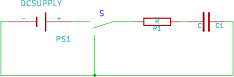
\includegraphics[width=2\textwidth/3]{figures/switch-circuit}
  \caption{The switching circuit used to discuss charging and
    discharging a capacitor.} 
  \label{fig:circuit}
\end{figure}
Since capacitors are used to store charge, we must find a way to
change the charge state on the capacitor.  Let's discuss the circuit
in Figure~\ref{fig:circuit}.  This circuit has three states:
\begin{inparaenum}
\item The steady state, where the switch is open, no current flows in
  the resistor, and the charge state on the capacitor is constant,
\item the ``charging'' state, where the battery or power supply is
  connected to the capacitor and adds charge to the capacitor, and
\item the ``discharging'' state, where the battery is disconnected,
  the two plates of the capacitor are connected to each other
  through the resistor, and removes charge from the capacitor.
\end{inparaenum}

We can analyze the dynamic states of the circuit using Kirchoff's
Rules:
\begin{enumerate}
\item The Loop rule (energy conservation) requires the sum of all
  voltages drops around a closed loop to vanish, and
\item The Junction rule (charge conservation) requires the sum of all
  currents into a junction to vanish.
\end{enumerate}
Let's apply these rules, first to the discharging and then to the
charging state:
\begin{enumerate}
\item Discharging: In the discharging case, the current will flow off
  the capacitor in a counter clockwise direction (why?).  When we
  close that switch, Kirchoff's rules become 
  \begin{align*}
    V_c - V_R &= 0\\
    -\deriv{q(t)}{t} - \frac{q(t)}{RC} &= 0\ .
  \end{align*}
  Again, the rate is negative, because the capacitor is discharging,
  not charging.  The method of solution for this equation is given in
  Appendix~\ref{sec:solutions}.
  \begin{gather*}
    V_c(t) = V_R(t) = V_s e^{-t/RC}\ ,
  \end{gather*}
  assuming that the initial voltage across the capacitor is $V_s$.
  This ``discharge curve'' is plotted in Figure~\ref{fig:curves}.
\item Charging: In the charging case, the current flows clockwise from
  the battery (at voltage $V_s$), through the resistor (at $V_R$), and
  across the capacitor $V_c$; we want to solve for $V_c$ as a function
  of time.  Kirchoff's Rules tell us
  \begin{align*}
    V_s - V_R - V_c &= 0\\
    V_s - I R - \frac{q}{C}\\
    \intertext{But here, the current through the resistor depends on
      the rate at which charge is changing on the capacitor; they have
      the same sign here since the charge on the capacitor is
      increasing}
    V_s - \deriv{q(t)}{t} R - \frac{q(t)}{C} &=0\\
    \deriv{q(t)}{t} + \frac{q(t)}{RC} &= \frac{V_s}{R}\ .
  \end{align*}
  We can solve this differential equation (see
  Appendix~\ref{sec:solutions}) for the time dependent voltage profile
  across the capacitor.  If we start with a completely discharged
  capacitor, the voltages across the resistors and capacitors vary as
  \begin{gather*}
    V_c(t) = V_s \left( 1 - e^{-t/RC} \right)\\
    V_R(t) = V_s e^{-t/RC}\ .
  \end{gather*}
  As the capacitor charges, the voltage across - and hence the
  charge on - the capacitor rises exponentially, while the voltage
  across - and hence the current through - the resistor will fall
  exponentially; see Figure~\ref{fig:curves}.
\end{enumerate}

\begin{figure}
  \centering
  \includegraphics[width=2\textwidth/3]{figures/curves}
  \caption{The capacitor charging and discharging curves}
  \label{fig:curves}
\end{figure}
The quantity $RC$ - which appears in the argument of the exponential -
is known as the \textit{time constant} of the system; it has units of
time, and determines the time interval over which voltages, charges,
and currents change in the circuit.  The time constant can be tuned by
modifying either $R$ or $C$.  In practice, more resistor than
capacitor values are commercially available, so it's easier to tune
the resistor values.

Given a known resistance we can measure the time constant of the $RC$
circuit, and algebraically determine the capacitance $C$.  When
discharging the capacitor,
\begin{gather*}
  V_c(t) = V_s e^{-t/RC}\ .
\end{gather*}
We can easily measure and use the half-life \halflife of the
discharge: \halflife is the time it takes for the voltage
to fall by half.  Substituting into the above equations and solving
for \halflife:
\begin{align*}
  \frac{V_s}{2} &= V_s e^{-\halflife/RC}\\
  \ln \frac{1}{2} &= -\frac{\halflife}{RC}\\
  \halflife &= \left(C \ln 2\right) R\ .
\end{align*}
If we allow $R$ to vary, then this equation defines a line with
abscissa $R$, ordinate \halflife, and slope $C \ln 2$.  If we measure
multiple $(R, \halflife)$ pairs, we can plot the data and fit them to
a line to extract the slope, and hence the capacitance.

\section{Procedures}
\label{sec:procedures}

You should receive an oscilloscope, a signal generator, a frequency
measuring multimeter, one unknown capacitor, a decade capacitance box,
and a decade resistance box.

\subsection{Time Constant of an RC Circuit}
\label{sec:timeconst}


\begin{figure}
  \centering
  \subfloat[][Measurement Circuit]{
    \label{fig:RCmeasuring:circuit}
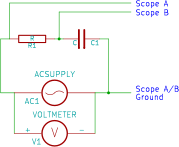
\includegraphics[width=\textwidth/3]{figures/measurement-circuit}
  } \qquad
  \subfloat[][Oscilloscope Display]{
    \label{fig:RCmeasuring:oscope}
    \includegraphics[width=\textwidth/3]{figures/oscope-trace}
  }
  \caption{The left-hand figure is the circuit used to measure the
    time constant of an RC circuit, while the right-hand figure shows
    the Oscilloscope traces.}
  \label{fig:RCmeasuring}
\end{figure}
In this part of the experiment, instead of a DC voltage and a
mechanical switch, we apply a square wave signal to the capacitor as
shown in Figure~\ref{fig:RCmeasuring}.  An ideal square wave has two
values: high and low (here $V_s$ and 0), and it switches between them
instantaneously.  The capacitor will charge when the voltage of the
square wave is $V_s$; the capacitor will discharge when the voltage of
the square wave is zero.  The oscilloscope traces of the charging and
discharging of the capacitor are also shown in
Figure~\ref{fig:RCmeasuring}.

It should be noted that if the period of the square wave $T_s$ is much
less than the time constant $\tau = RC$ ($T_s \ll \tau$), then the
capacitor will start discharging before it has sufficient time to
acquire the maximum charge $q_0$, making measurement of the time
constant difficult.  What will this look like on the oscilloscope?  If
$T_s$ is much more than $\tau$ ($T_s \gg \tau$), you will not be able
to fit both the charging and discharging portions of the capacitor
voltage on the oscilloscope trace at the same time.  Why?

\begin{enumerate}
\item Construct the circuit shown in
  Figure~\ref{fig:RCmeasuring:circuit}.
\item Perform the initial turn-on procedure for the oscilloscope (from
  the Cathode Ray Oscilloscope Lab).
\item Set the trigger mode to AUTO, vertical coupling to AC, and slope
  to ``+''.  To start, set both channels to $\unit[0.2]{V/div}$.  Make
  sure that the ground of both traces is at the same position on the
  screen. 
\item Start by setting the frequency of the square wave to about
  $\unit[100]{Hz}$ and the output voltage to $\unit[0.5]{V}$.
\item Adjust $R$ to about $\unit[8]{k\Omega}$, and $C$ to about
  $\unit[0.1]{\mu F}$.  What is the time constant of this combination?
\item Adjust the frequency of the square wave, and the time and
  voltage settings of the oscilloscope to obtain the traces as in
  Figure~\ref{fig:RCmeasuring:oscope}.  Measure and record $R$, $C$,
  $f$, $V$, \halflife, and the oscilloscope settings.
\item Measure the height of the decay curve at a number of points;
  switch the slope to ``-'', and measure the height of the charging
  curve at a number of points.  You will use these to map out the
  charging/discharging curves, and fit for the time constant.
\end{enumerate}

\subsection{Determine the Capacitance}
\label{sec:capacitance}

Here, we'll use the same techniques we just did to determine the value
of an unknown capacitor.

\begin{enumerate}
\item Replace the known capacitor with the unknown capacitor in the
  circuit.
\item Set the resistance to about $\unit[4]{k\Omega}$, and make the
  necessary adjustments to the oscilloscope settings to again obtain
  the appropriate display on the oscilloscope.
\item Measure and record $R$, $f$, $V$, the oscilloscope settings, and
  \halflife.
\item Repeat for four or five values of $R$; you need enough points to
  fit a line through your $(R,\halflife)$ pairs.
\end{enumerate}

\appendix

\section{Derivation of Solutions}
\label{sec:solutions}

The differential equations in Section~\ref{sec:theory} are the
simplest of all differential equations to solve: first order, linear
equations with constant coefficients.  Here, we'll solve a slightly
more complicated equation (a first order linear equation with
non-constant coefficients) in complete generality, and use this
solution to find the solutions we're interested in.  Consider the
following differential equation:
\begin{gather*}
  \deriv{y(x)}{x} + P(x) y(x) = Q(x)\ .
\end{gather*}
This equation looks very much like the equations we found in
Section~\ref{sec:theory} using Kirchoff's Rules.  We can solve this in
the following way.  First, we'll multiply both sides of this equation
by a new function, $M(x)$, and we'll first solve for $M(x)$.
\begin{gather*}
  M(x) \deriv{y(x)}{x} + M(x) P(x) y(x) = M(x) Q(x)\ .
\end{gather*}
Let's now assume that the left hand side is the expansion of the
product rule of $M(x) y(x)$:
\begin{gather*}
  \deriv{}{x} \left( M(x) y(x) \right) = M(x) Q(x)\ .
\end{gather*}
What must be true for this to hold?  Well,
\begin{gather*}
  \deriv{}{x} \left( M(x) y(x) \right) = 
  M(x) \deriv{y(x)}{x} + \deriv{M(x)}{x} y(x) = 
  M(x) \deriv{y(x)}{x} + M(x) P(x) y(x)\ .
\end{gather*}
This is true if and only if
\begin{gather*}
  \deriv{M(x)}{x} = M(x) P(x)\ .
\end{gather*}
This is a ``trivial'' problem to solve: just separate and integrate:
\begin{gather*}
  M(x) = e^{\int P(x) \dd x}\ .
\end{gather*}
Now, go a few lines back up the page:
\begin{gather*}
  \deriv{}{x} \left( M(x) y(x) \right) = M(x) Q(x)\ .
\end{gather*}
We can solve this one trivially, too, just by integrating
\begin{gather*}
  M(x) \left( y(x) -c \right) = \int^x M(x) Q(x) \dd x\ ,
\end{gather*}
where, since this is an indefinite integral, requires an integration
constant $c$.  Finally, then, we can solve the general problem:
\begin{gather*}
  y(x) = M(x)^{-1} \int^x M(x) Q(x) \dd x + c\ .
\end{gather*}

In the case of the charging RC circuit, $x = t$, $y(x) = q(t)$, $P(t)
= 1/RC$, and $Q(t) = V_s/R$.  Integrating gives us $M(t) = e^{t/RC}$,
giving us the solution:
\begin{align*}
  q(t) &= e^{-t/RC} \int_0^t e^{t/RC} \frac{V_s}{R} \dd t\\
  &= \frac{V_s}{R} RC e^{-t/RC} \left( e^{t/RC} -1 \right)\\
  &= V_s C \left( 1 - e^{-t/RC} \right)\ ,
\end{align*}
where we've used the integration constant to get the $t=0$ value right
(here, no charge on the capacitor).  Dividing both sides by $C$ gives
us the voltage across the capacitor at time $t$
\begin{gather*}
  V_c(t) = V_s \left( 1 - e^{-t/RC} \right)\ .
\end{gather*}

In the case of the discharging circuit, we have 
\begin{gather*}
  q(t) = V_s C e^{-t/RC}\ ,
\end{gather*}
where we assume the voltage across the capacitor at $t=0$ is $V_s$.
Again, divide by $C$ to get the voltage profile
\begin{gather*}
  V_c(t) = V_s e^{-t/RC}\ .
\end{gather*}

\newpage

\section*{Pre-Lab Exercises}

Answer these questions as instructed on Blackboard; make sure to
submit them before your lab session!

\begin{enumerate}
\item What is the time constant for an RC circuit with $R =
  \unit[45]{k\Omega}$ and $C = \unit[1.2]{\mu F}$?
\item If it takes $\unit[5]{\mu s}$ for a capacitor to charge to half
  the battery voltage, through a $\unit[10]{k|omega}$ resistor, what
  is the capacitance $C$?
\item A given RC circuit charges through a particular resistor $R$,
  and capacitor, $C$.  If I double the capacitance, what happens to
  the time constant?  What if I double the resistance?
\end{enumerate}

\newpage

\section*{Post-Lab Exercises}

\begin{enumerate}
\item Determine the time constant of the RC circuit with known
  capacitance.  Do this by plotting your data of time versus the
  amplitude of the signal.  You should fit this data to an
  exponential, and extract $\tau$.  There are a number of ways to do
  this:
  \begin{inparaenum}
  \item use a mathematics package capable of sophisticated statistical
    analysis, such as R, Octave, Matlab, Mathematica, etc., or
  \item using a spreadsheet, you can transform your data into a linear
    function, and fit that in Excel using a trendline analysis.
  \end{inparaenum}
  Estimate the uncertainty of this measured time constant.  You should
  also estimate the time constant from the measured \halflife.  Do
  these multiple experimental extractions agree within your estimated
  uncertainty?  Do they agree with the theoretical expectation?
\item Determine the unknown capacitance.  Plot your $(R, \halflife)$
  data pairs, and fit the data to a line.  Extract the capacitance
  from the fitted line parameters.  Estimate the uncertainty of this
  extracted capacitance.  You can also estimate the capacitance from
  the individual $(R, \halflife)$ pairs; estimate your uncertainties.
  Do these estimates agree with the line fit estimate?
\item Discuss briefly whether you have met the objectives of the lab
  exercises.
\end{enumerate}

\end{document}

%%% Local Variables: 
%%% mode: latex
%%% TeX-master: t
%%% End: 
